\documentclass[11pt, oneside]{article} 
\usepackage{geometry}
\geometry{letterpaper} 
\usepackage{graphicx}
	
\usepackage{amssymb}
\usepackage{amsmath}
\usepackage{parskip}
\usepackage{color}
\usepackage{hyperref}

\graphicspath{{/Users/telliott/Github/figures/}}
% \begin{center} 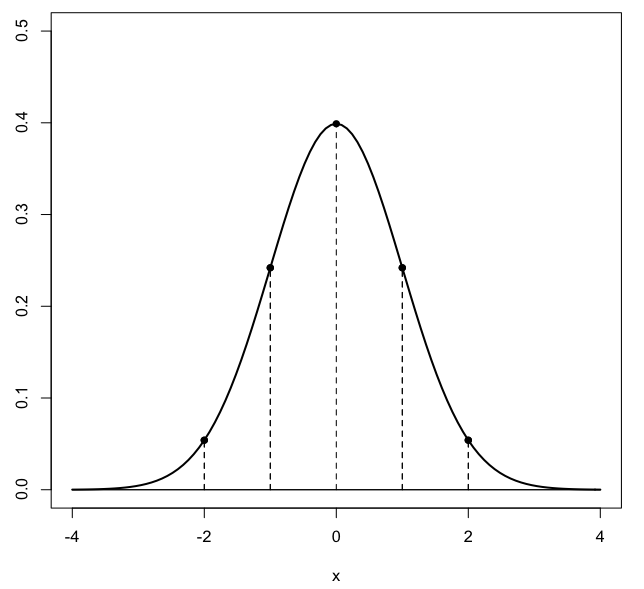
\includegraphics [scale=0.4] {gauss3.png} \end{center}

\title{Sum of angles}
\date{}

\begin{document}
\maketitle
\large

\subsection*{cosine of a sum}

The sum of angle formulas (for the sine and cosine of the sum or difference of two angles) are used often in calculus, not only for solving problems, but even in finding an expression for the derivative of sine and cosine.

You really must know them.  I think it's so important that we will show several ways of finding these formulas.  The easiest way to remember them uses Euler's equation.  We'll see that at the end.

There are four equations, one each for $\sin s \pm t$ and $\cos s \pm t$.

I've memorized only one:
\[ \cos s - t = \cos s \cos t + \sin s \sin t \]

By $\cos s - t$ we mean $\cos (s - t)$, but have left off the parentheses.  Say "cos cos" and then recall the difference in sign, minus on the left, plus on the right.

\subsection*{check with $s = t$}

I like this version because it can be checked easily.  Just set $s = t$:
\[ \cos s - t = \cos s - s = \cos 0 = 1 = \cos^2 s + \sin^2 s \]
which is our favorite trigonometric identity and obviously correct.

\subsection*{derivation 0}
I'm calling this one derivation zero because it was added later, and it is really a simplified form of derivation 1.  We draw two triangles one on top of the other, with the hypotenuse of the second scaled to be equal to $1$.  Then draw a rectangle around the whole thing.

\begin{center} \includegraphics [scale=0.4] {sum_angles_6.png} \end{center}

So first of all, for the triangle with angle $\theta$ and hypotenuse $1$, the labels should be obvious.

Second, for triangles with angle $\phi$ where the hypotenuse is \emph{not} $1$, we have something like $\cos \phi \cos \theta$ on the bottom of the figure, which gives the desired value $\cos \phi$ after dividing by the hypotenuse, $\cos \theta$.

Finally, the angle labeled $\theta + \phi$ at the top is known by the alternate interior angles theorem.

Just read off the relationships from the sides of the rectangle:
\[ \sin \phi + \theta = \sin \phi \cos \theta + \cos \phi \sin \theta \]
\[ \cos \phi + \theta = \cos \phi \cos \theta - \sin \phi \sin \theta \]

And what's really nice is that a simple change will give the difference formulas:

\begin{center} \includegraphics [scale=0.4] {sum_angles_7.png} \end{center}
We've changed the symbol $\phi$ to refer to the complementary angle for what it was before.  As a result, by alternate interior angles, the two angles $\theta - \phi$ and $\theta$ together, are equal to $\phi$.  Switch the labels appropriately (it's easy since this $\phi$ is the complement of the old one).

Read the result:
\[ \sin \phi - \theta = \sin \phi \cos \theta - \cos \phi \sin \theta \]
\[ \cos \phi - \theta = \cos \phi \cos \theta + \sin \phi \sin \theta \]

\subsection*{derivation 1}

Here is a geometric derivation of the sum of angles formulas for both sine and cosine.  The key is to draw an inspired diagram.

Construct a right triangle, with one of the smaller angles labeled $s$.  Then construct another right triangle with small angle $t$, with the hypotenuse of the first triangle containing angle $s$ as the base adjacent to angle $t$ in the second triangle, placing them one on top of the other as shown:

\begin{center} \includegraphics [scale=0.4] {sum_angles_3.png} \end{center}
Scale the combined triangles so that the hypotenuse of the second triangle has unit length.

Our crucial insight is to draw vertical and horizontal dotted lines as shown in the right panel.

But first, notice that the angle $\phi$ is part of two different right triangles.  One has base angle $s + t$ with $s + t + \phi = \pi/2$.  The other has base angle $t$ with $t + \phi + s' = \pi/2$.

Clearly $s = s'$. So change the label on that angle.  The small triangle with dotted lines for the bases and the angle now labeled $s$ is similar to the first triangle we drew.

Next, add some labels to the sides of the triangles.
\begin{center} \includegraphics [scale=0.4] {sum_angles_4.png} \end{center}

The first two labels are easy because the length of the hypotenuse of the top triangle is $1$, so the opposite side is $\sin t$ and the adjacent side is $\cos t$.

For the next part, we need to remember what happens if the hypotenuse is \emph{not} $1$.  Recall that in a circle of radius $r$ we write $x = r \cos \theta$ for the side adjacent to the central angle.  That's so it will cancel when we form the ratio with the hypotenuse of length $r$.

In the same way, the adjacent side in the triangle with small angle $s$ is $\cos s \cos t$, so that when divided by the hypotenuse $\cos t$ it gives the correct result, namely, $\cos s$.  

\begin{center} \includegraphics [scale=0.4] {sum_angles_5.png} \end{center}

This explains why the sides of the small triangle with angle $s$ at the top are labeled as $\sin s \sin t$ and $\cos s \sin t$.  When divided by the hypotenuse of length $\sin t$, they give the correct result for the ratio.  The side opposite angle $s$ ($\sin s \cos t$) is explained in the same way.

We're nearly done.  We simply have to look for $\cos s + t$ and $\sin s + t$ in the figure.  Use the long vertical dotted line to form the right triangle with base angle $s + t$.  

I claim that the two parts of the base are $\cos s + t$ and $\sin s \sin t $ and they add to give:
\[ \cos s + t + \sin s \sin t = \cos s \cos t \]
which rearranges to
\[ \cos s + t = \cos s \cos t - \sin s \sin t \]
Similarly, the entire dotted vertical is $\sin s + t$, composed of these two parts: 
\[ \sin s + t = \sin s \cos t + \cos s \sin t \]

\subsection*{change signs}

For $\cos s - t$, flip the sign on the second term.  
\[ \cos s - t = \cos s \cos t + \sin s \sin t \]
That's because
\[ \cos -\theta = \cos \theta \]
\[ \sin - \theta = - \sin \theta \]

\begin{center} 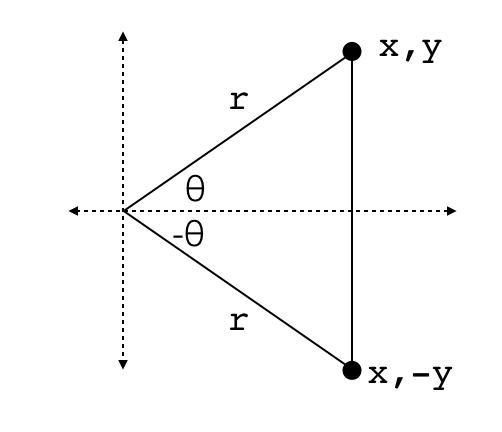
\includegraphics [scale=0.4] {pm_theta.png} \end{center}

The diagram shows the reason:
\[ \cos \theta = x/r = \cos - \theta \]
while
\[ \sin \theta = y/r = -  (\sin - \theta ) = - (-y/r) \]

Substitute $- \sin \theta$ for $\sin - \theta$ and $\cos \theta$ for $\cos - \theta$:
\[ \cos s - t = \cos s \cos - t + \sin s \sin - t \]
\[ = \cos s \cos t - \sin s \sin t \]
and
\[ \sin s - t = \sin s \cos t - \cos s \sin t \]

\subsection*{derivation 2 (Strang)}

For a geometric derivation of the sum of angles formula with minimal setup, I really like this figure from Strang

\begin{center} 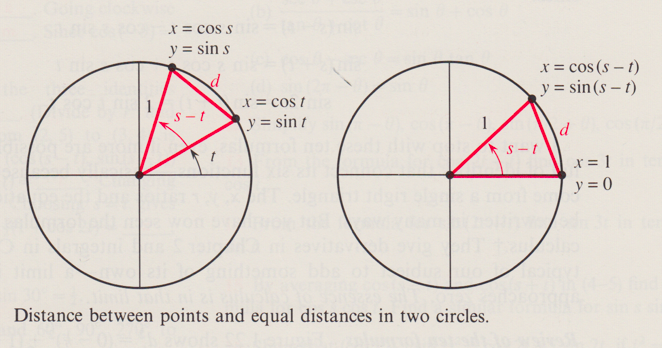
\includegraphics [scale=0.6] {strang_sum.png} \end{center}

We have the same triangle in the two panels, just rotated clockwise on the right.

The squared distance between two points in the plane is
\[ d^2 = (x_2 - x_1)^2 + (y_2 - y_1)^2 = \Delta x^2 + \Delta y^2 \]
This is just the Pythagorean theorem in disguise.

In the left panel, $t$ is the angle between the lower radius and the $x$-axis, $s$ is the angle between the upper radius and the $x$-axis, and as labeled, $s-t$ is the angle between the two radii.

The distance $d$ squared for the two points on the circle in the left panel is
\[ d^2 = (\cos s - \cos t)^2 + (\sin s - \sin t)^2 \]

Multiply out:
\[ d^2 = \cos^2 s - 2 \cos s \cos t  + \cos^2 t +  \sin^2 s - 2 \sin s \sin t + \sin^2 t \]
We have two copies of $\sin^2 + \cos^2$, one for angle $s$  and one for angle $t$
\[ d^2 = 2 - 2 \cos s \cos t - 2 \sin s \sin t \]

In the right panel, the two radii have been rotated, preserving the same angle between them.
\[  d^2 = (\cos (s-t) - 1)^2 + \sin(s-t)^2 \]
(Don't forget the $1$).
\[ = \cos^2 (s-t) - 2 \cos(s-t) + 1 + \sin^2 (s-t) \]
\[ = 2 - 2 \cos(s-t) \]

Because the included angle hasn't changed, neither has the distance, so we can equate the two expressions.  
\[ 2 - 2 \cos(s-t) = 2 - 2 \cos s \cos t - 2 \sin s \sin t \]
Subtract 2 from both sides, divide by $2$, and change all the signs leaving
\[ \cos (s - t) = \cos s \cos t + \sin s \sin t \]
This is our formula for the cosine of the difference of two angles.

The disadvantage of this construction is that there is no easy way to get the formula for sine.  That brings us to some tricky computations.

\subsection*{getting to sine}

Look at the relationships between sine and cosine for angles that are related by addition or subtraction of $\pi/2$.
\begin{center} 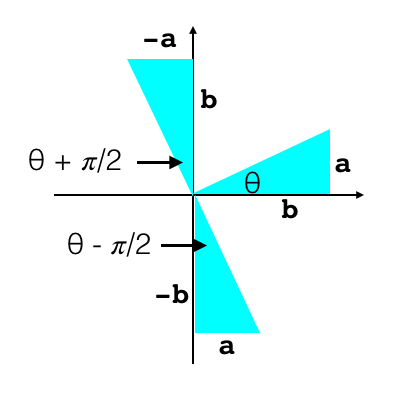
\includegraphics [scale=0.4] {angles2.png} \end{center}
In the figure, I have simply rotated the same triangle.

From the figure we can easily read off these four identities
\[ \sin (\theta + \pi/2) = b = \cos \theta \]
\[ \cos (\theta + \pi/2) = -a = -\sin \theta \]
And
\[ \sin (\theta - \pi/2) = - b = -\cos \theta \]
\[ \cos (\theta - \pi/2) = a = \sin \theta \]

Here is an alternative derivation which proceeds from the graph of sine and cosine versus the angle.

\begin{center} 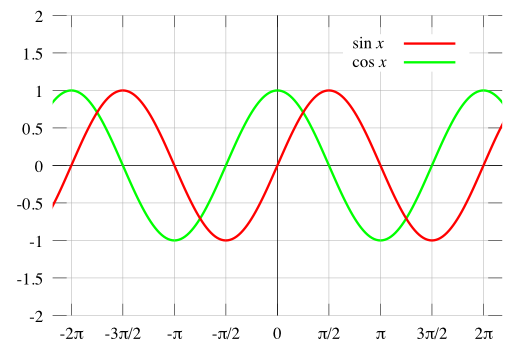
\includegraphics [scale=0.4] {sine_cosine_wikipedia.png} \end{center}

Pick some angle (say $\theta = 0$), then $\cos \theta = 1$.  What is the angle for which the sine gives the same result?  The sine curve is exactly like the cosine, it is just shifted to the right by a \emph{phase change} of $\pi/2$. 

That angle is $\theta + \pi/2$.  The phase change is added to the angle:
\[ \cos \theta = \sin (\theta + \frac{\pi}{2}) \]

Try the same reasoning in reverse.  The cosine curve is exactly like the sine, it is just shifted by a phase change of $-\pi/2$, i.e. to the left.  

Pick some angle (say $\theta = \pi/2$), then $\sin \theta = 1$.  What is the value of the angle for which the cosine gives the same result?  It is $\theta - \pi/2$.  The phase change is subtracted from the angle $\theta$:
\[ \sin \theta = \cos (\theta - \frac{\pi}{2}) \]

In summary, switching sine for cosine gives a valid expression, but there is a difference of \emph{sign} for the phase.

\subsection*{back to our task}

We had
\[ \cos (s - t) = \cos s \cos t + \sin s \sin t \]
Let
\[ u = t - \frac{\pi}{2}, \ \ \ \ \ \  t  = u + \frac{\pi}{2} \]

Substitute for $t$
\[ \cos \ [ \ s - (u + \frac{\pi}{2}) \ ] \ = \cos s \cos (u + \frac{\pi}{2}) + \sin s \sin (u + \frac{\pi}{2}) \]
Regroup the left-hand side
\[ \cos \ [ \ (s - u) - \frac{\pi}{2}) \ ] \ = \cos s \cos (u + \frac{\pi}{2}) + \sin s \sin (u + \frac{\pi}{2}) \]

Referring to the results we obtained above, cosine something minus $\pi/2$ is the sine of that something:
\[ \sin (s - u) = \cos s \cos (u + \frac{\pi}{2}) + \sin s \sin (u + \frac{\pi}{2}) \]
Cosine something plus $\pi/2$ is minus the sine:
\[ \sin (s - u) = -\cos s \sin u + \sin s \sin (u + \frac{\pi}{2}) \]
Sine something plus $\pi/2$ is cosine:
\[ \sin (s - u) = -\cos s \sin u + \sin s \cos u \]

Rearrange:
\[ \sin (s - u) = \sin s \cos u - \sin u \cos s \]

This is correct, but the path is fraught with error!  

\subsection*{derivation 3}
There is another easy derivation based on rotation of unit vectors.  But you need to understand a bit about matrix multiplication for that.  Basically the idea is that a point $x,y$ in the plane can be represented as a vector:
\[ 
\begin{bmatrix}
x \\
y
\end{bmatrix}
\]
Rotation of the vector amounts to multiplication by a matrix
\[
\begin{bmatrix}  
\cos \theta & -\sin \theta \\
\sin \theta & \ \  \cos \theta 
\end{bmatrix}
\begin{bmatrix}  x \\ y \end{bmatrix}
=
\begin{bmatrix}  u \\ v \end{bmatrix}
\]

To explain where this matrix comes from, we have to think about rotation of the unit vectors $\hat{\mathbf{i}}$ (in the $x$-direction) and $\hat{\mathbf{j}}$ (in the $y$-direction) through an angle $\theta$ counter-clockwise.  

Start with $\hat{\mathbf{i}}$.  The new vector we seek is still a unit vector, but rotated so that it forms an angle $\theta$ with the positive $x$-axis.

The new vector has both $\hat{\mathbf{i}}$ and $\hat{\mathbf{j}}$ components. Projection onto $\hat{\mathbf{i}}$ gives a vector with unit length times $\cos \theta$, that is,  just $\cos \theta$.  Similarly, the projection onto $\hat{\mathbf{j}}$ gives a length $\sin \theta$.  The squared length is $\cos^2 \theta + \sin^2 \theta$, so this really is a unit vector.

In vector notation we would say that
\[ \langle 1,0 \rangle \ \Rightarrow \ \langle \cos \theta, \sin \theta \rangle \]
In matrix language the two vectors are related in this way:
\[
\begin{bmatrix}  
1  \\  
0  
\end{bmatrix}
\Rightarrow
\begin{bmatrix}  
\cos\  \theta  \\  
\sin\  \theta  
\end{bmatrix}
\]
where $\Rightarrow$ refers to rotation.

So the question is, what matrix will multiply $\hat{\mathbf{i}}$ to give this result?
\[
\begin{bmatrix}  
a & b  \\  
c & d  
\end{bmatrix}
\begin{bmatrix}  
1  \\  
0  
\end{bmatrix}
=
\begin{bmatrix}  
\cos\  \theta  \\  
\sin\  \theta  
\end{bmatrix}
\]
Matrix multiplication works like this
\begin{center} 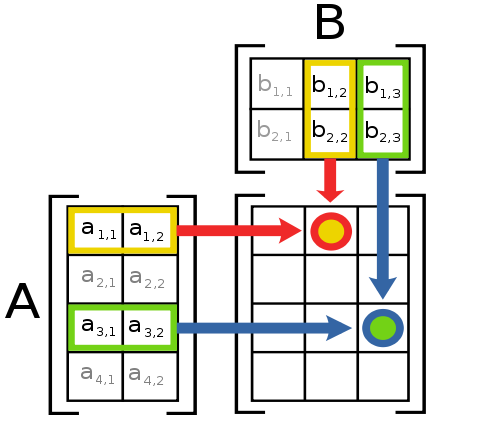
\includegraphics [scale=0.35] {mm1.png} \end{center}
The entry in row $r$ and column $c$ of the result is formed by doing a special operation on row $r$ of the matrix, times column $c$ of the second.  For a matrix times a vector, the result is also a vector, with only a single column.

The operation is called the dot product.  For the red entry in the figure:
\[ (a_{11},a_{12}) \cdot (b_{21},b_{22}) = a_{11}b_{21} + ,a_{12}b_{22} \]

So going back to this:

\[
\begin{bmatrix}  
a & b  \\  
c & d  
\end{bmatrix}
\begin{bmatrix}  
1  \\  
0  
\end{bmatrix}
=
\begin{bmatrix}  
\cos\  \theta  \\  
\sin\  \theta  
\end{bmatrix}
\]


I hope it's pretty clear that $a = \cos \theta$ and $c = \sin \theta$:
\[
\begin{bmatrix}  
\cos \theta & b  \\  
\sin \theta & d  
\end{bmatrix}
\begin{bmatrix}  
1  \\  
0  
\end{bmatrix}
=
\begin{bmatrix}  
\cos\  \theta  \\  
\sin\  \theta  
\end{bmatrix}
\]
Can you see why this is true?  Since the $y$-component of the unit vector $\hat{\mathbf{i}}$ is zero, we have no information for the moment about what $b$ and $d$ will be.

On the other hand, rotation of the unit $\hat{\mathbf{j}}$ vector by $\theta$ should give
\[
\begin{bmatrix}  
a & b  \\  
c & d  
\end{bmatrix}
\begin{bmatrix}  
0  \\  
1  
\end{bmatrix}
=
\begin{bmatrix}  
-\sin \  \theta  \\  
\ \ \cos \  \theta  
\end{bmatrix}
\]
The minus sign comes because the new unit vector is now sticking out into the second quadrant.

\begin{center} 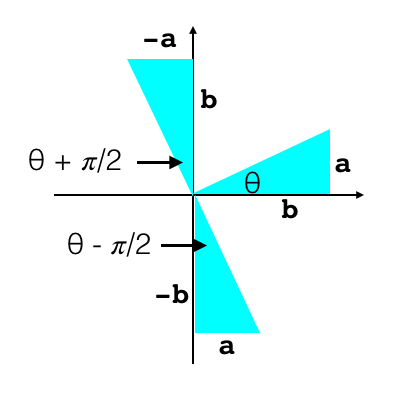
\includegraphics [scale=0.4] {angles2.png} \end{center}

Again, it should be clear that 
\[
\begin{bmatrix}  
a & -\sin \  \theta  \\  
c & \ \ \cos \  \theta  
\end{bmatrix}
\begin{bmatrix}  
0  \\  
1  
\end{bmatrix}
=
\begin{bmatrix}  
-\sin \  \theta  \\  
\ \ \cos \  \theta  
\end{bmatrix}
\]

Now, just put them together:
\[
R_{ccw} = 
\begin{bmatrix}   \ \cos \theta & -\sin \theta  \\  \ \sin \theta & \ \ \cos \theta  \end{bmatrix}
\]
This is called a \emph{rotation matrix}.  It rotates vectors.

\[
\begin{bmatrix}   \ \cos \theta & -\sin \theta  \\  \ \sin \theta & \ \ \cos \theta  \end{bmatrix}
\begin{bmatrix}   x   \\  y  \end{bmatrix} = \begin{bmatrix}   u   \\  v  \end{bmatrix}
\]
In particular, a rotation of $90^{\circ}$ ccw goes like this
\[
\begin{bmatrix}   0 & -1  \\  1 & \ \ 0  \end{bmatrix}
\begin{bmatrix}   1   \\  0  \end{bmatrix} = \begin{bmatrix}   0   \\  1  \end{bmatrix}
\]
$\hat{\mathbf{i}}$ is rotated to become $\hat{\mathbf{j}}$.

\[
\begin{bmatrix}   0 & -1  \\  1 & \ \ 0  \end{bmatrix}
\begin{bmatrix}   0   \\  1  \end{bmatrix} = \begin{bmatrix}   -1   \\  0  \end{bmatrix}
\]
$\hat{\mathbf{j}}$ is rotated to become $-\hat{\mathbf{i}}$.

I claim that since the matrix we found works for both of the unit vectors it will work for any vector, because any vector can be written as a linear combination of the unit vectors
\[ \mathbf{a} = a_1 \ \hat{\mathbf{i}} + a_2 \ \hat{\mathbf{j}} \]

The inverse of the matrix we derived would be used for clockwise rotation and it is just
\[
R_{cw} =
\begin{bmatrix}   \ \ \ \cos \theta & \ \sin \theta  \\  -\sin \theta & \ \ \cos \theta  \end{bmatrix}
\]
You can verify this by remembering the rule for $2 \times 2$ or by multiplication
\[
R_{cw} \  R_{ccw} =
\begin{bmatrix}   \ \ \ \cos \theta & \ \sin \theta  \\  -\sin \theta & \ \ \cos \theta  \end{bmatrix}
\begin{bmatrix}   \ \cos \theta & -\sin \theta  \\  \ \sin \theta & \ \ \cos \theta  \end{bmatrix}
= 
\begin{bmatrix}   1 & 0  \\  0 & 1 \end{bmatrix}
= I
\]
Don't be confused when someone talks about rotation of the coordinate system.  Here, the coordinate system stayed fixed but we rotated the vector counter-clockwise.  We achieve the same thing (and use the same equation) for a \emph{clockwise} rotation of the coordinate system through an angle $\theta$.

\begin{center} 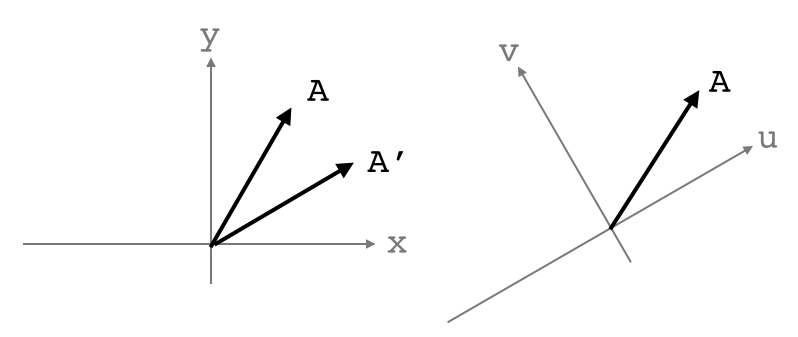
\includegraphics [scale=0.4] {rotate_vec_coord.png} \end{center}

If you really want to rotate the coordinate system counter-clockwise, rotate the vector clockwise.

\subsection*{consequence}

Something great comes out of this when we ask about rotation by the combined angle $s + t$.  

We can write two equivalent expressions, one by substituting $\theta=s+t$, and the other by doing two sequential applications of the matrix.  That is:
\[
\begin{bmatrix}   \ \cos (s+t) & -\sin (s+t)  \\  \ \sin (s+t) & \ \ \cos (s+t)  \end{bmatrix} =
\begin{bmatrix}   \ \cos s & -\sin s  \\  \ \sin s & \ \ \cos s  \end{bmatrix}
\begin{bmatrix}   \ \cos t & -\sin t  \\  \ \sin t & \ \ \cos t  \end{bmatrix}
\]
Look at the term on the upper-left, $\cos(s+t)$.  Sound familiar?  Carry out the matrix multiplication on the right for that element
\[ \cos(s+t) = \cos s \cos t - \sin s \sin t \]
We have derived the cosine addition formula.  Similarly, the bottom-left term is for the sine
\[ \sin(s+t) = \sin s \cos t + \cos s \sin t \]

\subsection*{yet another way}
We can look at this in still a different way.  Write
\[
\begin{bmatrix}  x \\ y \end{bmatrix}
=
x
\begin{bmatrix}  1 \\ 0 \end{bmatrix}
+
y
\begin{bmatrix}  0 \\ 1 \end{bmatrix}
\]
In this representation, the vector $\langle x,y \rangle$ is a linear combination of the unit vectors $\mathbf{\hat{i}} =\ \langle 1,0 \rangle$ and $\mathbf{\hat{j}}  =\ \langle 0,1 \rangle$.

To rotate the point, we just want to use a different set of unit vectors.  The new unit vectors (for the rotated axes) are $\langle \cos \theta,\sin \theta \rangle$ and $\langle -\sin \theta,\cos \theta \rangle$.  

If you compute their lengths, it is clear that they are, in fact, unit vectors.
\[
\begin{bmatrix}  x' \\ y' \end{bmatrix}
=
x
\begin{bmatrix}  \cos \theta \\ \sin \theta \end{bmatrix}
+
y
\begin{bmatrix}  -\sin \theta \\ \ \ \cos \theta \end{bmatrix}
\]
Written as a matrix multiplication, this is
\[
\begin{bmatrix}  x' \\ y' \end{bmatrix}
=
\begin{bmatrix}  
\cos \theta & -\sin \theta \\
\sin \theta & \ \  \cos \theta 
\end{bmatrix}
\begin{bmatrix}  x \\ y \end{bmatrix}
\]

That's what we said!

\subsection*{derivation 4}
Here is another setup, for rotation of the coordinate system.
\begin{center} \includegraphics [scale=0.4] {min_rotation2.png} \end{center}

\[ u = u_1 + u_2 = x \cos t + y \sin t \]
\[ v = v_1 - v_2 = y \cos t - x \sin t  \]

There is a change of sign with respect to the previous equations.  The reason is that here we have rotated the coordinate system counter-clockwise.  That's the same as rotating the point clockwise.

Although it's short and sweet, in my experience the geometry of this proof is very difficult to remember.

Shankar uses a very similar diagram.

To obtain the addition formulas, imagine that we rotate first through angle $s$ and then through angle $t$.  For the first
\[ x' = x \cos s + y \sin s \]
\[ y' = - x \sin s + y \cos s \]
(We use primes because there will be two rotations).

For the second
\[ x'' = x' \cos t + y' \sin t \]
\[ = (x \cos s + y \sin s) \cos t + (-x \sin s + y \cos s) \sin t \]
and
\[ y'' = - x' \sin t + y' \cos t \]
\[ y'' = -(x \cos s + y \sin s) \sin t + (-x \sin s + y \cos s) \cos t \]

Multiply through:
\[ x'' = x \cos s \cos t + y \sin s \cos t - x \sin s \sin t + y \cos s \sin t \]
\[ y'' = -x \cos s \sin t - y \sin s \sin t - x \sin s \cos t + y \cos s \cos t \]

And now the key is that we must have equality with
\[ x'' = x \cos (s + t) + y \sin (s + t) \]

The $x$ and $y$ terms must match.  So that means:
\[ \cos (s + t) = \cos s \cos t - \sin s \sin t \]
\[ \sin (s + t) = \sin s \cos t + \cos s \sin t \]
We obtain exactly the same expressions from either $x''$ or $y''$.

\subsection*{derivation 5 (Euler)}
Euler's formula is:
\[ e^{i \theta} = \cos \theta + i \sin \theta \]

If you've never seen it before, don't worry what it means or where it comes from.  Just treat $i$ as a constant with $i^2 = -1$.  Multiply as follows:
\[ (\cos s + i \sin s)(\cos t + i \sin t) \]
\[ = \cos s \cos t + i^2 \sin s \sin t + i \ [ \ \sin s \cos t + \cos s \sin t \ ] \] 
\[ = \cos s \cos t - \sin s \sin t + i \ [ \ \sin s \cos t + \cos s \sin t \ ] \] 

This is a \emph{complex} number with a real part (the first two terms), plus an imaginary part, the last two terms, with a leading factor of $i$.

For the same calculation with the exponential
\[ e^{is} \cdot e^{it} = e^{i(s+t)} \]
\[ = \cos (s + t) + i \sin (s + t) \]

By Euler's formula, these two expressions are equal.  

The rule for equality of complex numbers is that both the real parts and the imaginary parts must be equal.  So we have
\[ \cos (s + t) = \cos s \cos t - \sin s \sin t \]
\[ \sin (s + t) = \sin s \cos t + \cos s \sin t \]

\subsection*{double-angle formulas}
Very quickly, sine:
\[ \sin s + t = \sin s \cos t + \cos s \sin t \]
\[ \sin 2t = 2 \sin t \cos t \]
And cosine:
\[ \cos s + t = \cos s \cos t - \sin s \sin t \]
\[ \cos 2t = \cos^2 t - \sin^2 t = 2 \cos^2 t - 1 \]

Sometimes, it is helpful to have a simpler notation.  If we write $S$ for sine and $C$ for cosine, and use a prime for the double angle:
\[ S' = 2SC \]
\[ C' = 2C^2 - 1 \]
The inverse tangent is
\[ \frac{1}{T'} = \frac{1}{T} - \frac{1}{2SC} = \frac{1}{T} - \frac{1}{S} \]

\subsection*{geometric derivation}

Here is a simple geometric derivation of the double angle formula for sine.

\begin{center} \includegraphics [scale=0.4] {double_angle.png} \end{center}

From our work with arcs, we know that angle $\phi$ on the left is one-half the central angle $\theta$, and from Thales' theorem, that the angle on the circle at the top-right is a right angle.  So the angle in the triangle with sides $x-y-h$ is also $\phi$, as labeled, since they have the same complementary angle.

It helps to know where we're going, as well.  From above:
\[ \sin 2t = 2 \sin t \cos t \]
\[ \sin \theta = 2 \sin \phi \cos \phi \]

Now, $\sin \theta$ is just $y/1 = y$.  From the diagram:
\[ 2 \sin \phi \cos \phi = 2 \ \frac{xy}{h^2} = 2 \ \frac{xy}{x^2 + y^2} \]

\begin{center} \includegraphics [scale=0.4] {double_angle.png} \end{center}

But using the Pythagorean theorem, from the triangle with hypotenuse $1$ we know that
\[ (1 - x)^2 + y^2 = 1 \]
\[ 1 - 2x + x^2 + y^2 = 1 \]
\[ x^2 + y^2 = 2x \]

Substituting into the previous result:
\[ 2 \sin \phi \cos \phi = 2 \frac{xy}{2x} = y = \sin \theta \]

$\square$

The same diagram will serve for the cosine.  From the double-angle formula:
\[ \cos \theta = 2 \cos^2 \phi - 1 = 2 \ \frac{y^2}{x^2 + y^2} - 1 \]
since we had $x^2 + y^2 = 2x$ above:
\[ \cos \theta = 1 - x = \frac{y^2}{x} - 1 \]
\[ x - x^2 = y^2 - x \]
Rearrange to obtain the same identity again.  It checks.

$\square$

\subsection*{another calculation}
We found previously that 
\[ \sin \frac{\pi}{4} = \cos \frac{\pi}{4} = \frac{1}{\sqrt{2}} \]
\[ \sin \frac{\pi}{6} = \cos \frac{\pi}{3} = \frac{1}{2}; \ \ \ \ \sin \frac{\pi}{3} = \cos \frac{\pi}{6} = \frac{\sqrt{3}}{2} \]

These angles correspond to 30, 45 and 60 degrees.  It might be nice to have sine and cosine of 15 and 75 degrees as well.  That would make even divisions of the first 90 degrees.  We can get them as the sum and difference of $\pi/4$ and $\pi/6$.

Let $s = \pi/4$ and $t = \pi/6$.  Then

\[ \sin \frac{\pi}{12} = \sin s - t = \sin s \cos t - \sin t \cos s \]
\[ = \frac{1}{\sqrt{2}} \cdot \frac{\sqrt{3}}{2} - \frac{1}{2} \cdot \frac{1}{\sqrt{2}} = \frac{\sqrt{3} - 1}{2 \sqrt{2}} \]
\[ \cos \frac{\pi}{12} = \cos s - t = \cos s \cos t + \sin s \sin t \]
\[ = \frac{\sqrt{3}}{2} \cdot \frac{1}{\sqrt{2}} - \frac{1}{2} \cdot \frac{1}{\sqrt{2}} = \frac{\sqrt{3} + 1}{2 \sqrt{2}} \]

We just check that $\sin^2 \theta + \cos^2 \theta = 1$:
\[ \frac{(\sqrt{3} - 1)^2 + (\sqrt{3} + 1)^2}{(2 \sqrt{2})^2} \]
\[ = \frac{3 - 2 \sqrt{3} + 1 + 3 + 2 \sqrt{3} + 1}{8} = 1 \]

We can calculate similarly for $s + t = 5 \pi/12$ or just switch sine and cosine from $\pi/12$.

\end{document}